\section{Tuesday, March 19th}
\subsection{Logistics}
\begin{enumerate}
    \item Peer Review -- due Thursday.
    \item Chapter 4 Reading posted
    \item Quiz 5 retake will be on Wednesday 5:00pm
\end{enumerate}
\subsection{Goals}
\begin{itemize}
    \item Bayes Optimal Experimental Design: 
\end{itemize}
\begin{shaded}
Information is \underline{expected $\Delta$ in dist. of unknown after observation}.
\end{shaded}


\subsection{Problem}
\begin{itemize}
    \item $X\in\R^d$ is some unknown
    \begin{itemize}
        \item \underline{a priori}: $X\sim p_0$
    \end{itemize}
    \item have a set of questions $Q=\{q_j\}_{j=1}^m$ where, when we ask $q_j\to$ observe $Y$\\
($Y$ is a measurement, it has noise)
    \item \textbf{each $q$ is expensive}
\end{itemize}


\begin{itemize}
    \item \underline{Aim}: design a protocol for choosing an optimal sequence of questions... $\{q_{j(n)}\}_{n=1}^{\cdots}$
    \begin{itemize}
        \item \underline{Greedy}: choose $q_{j(n)}$ given the initial distribution for $x$ (which is $p_0$) \underline{and} everything we have learned so far: $Y^{(n-1)}=[Y_1, Y_2, \ldots, Y_{n-1}]$
    \end{itemize}
\end{itemize}


We are often trying to find answers to continuous problems (Huffman was greedy in reverse --  it worked by saving your question for the last 2 things -- you build your tree backwards). Thus since there are an uncountable infinity amount of outcomes, we can't start backwards -- we cannot use Huffman.

Since the Fano question is at most 2 questions (2 bits) worse than Huffman, we note that it is decent.

\begin{figure}[H]
    \centering
    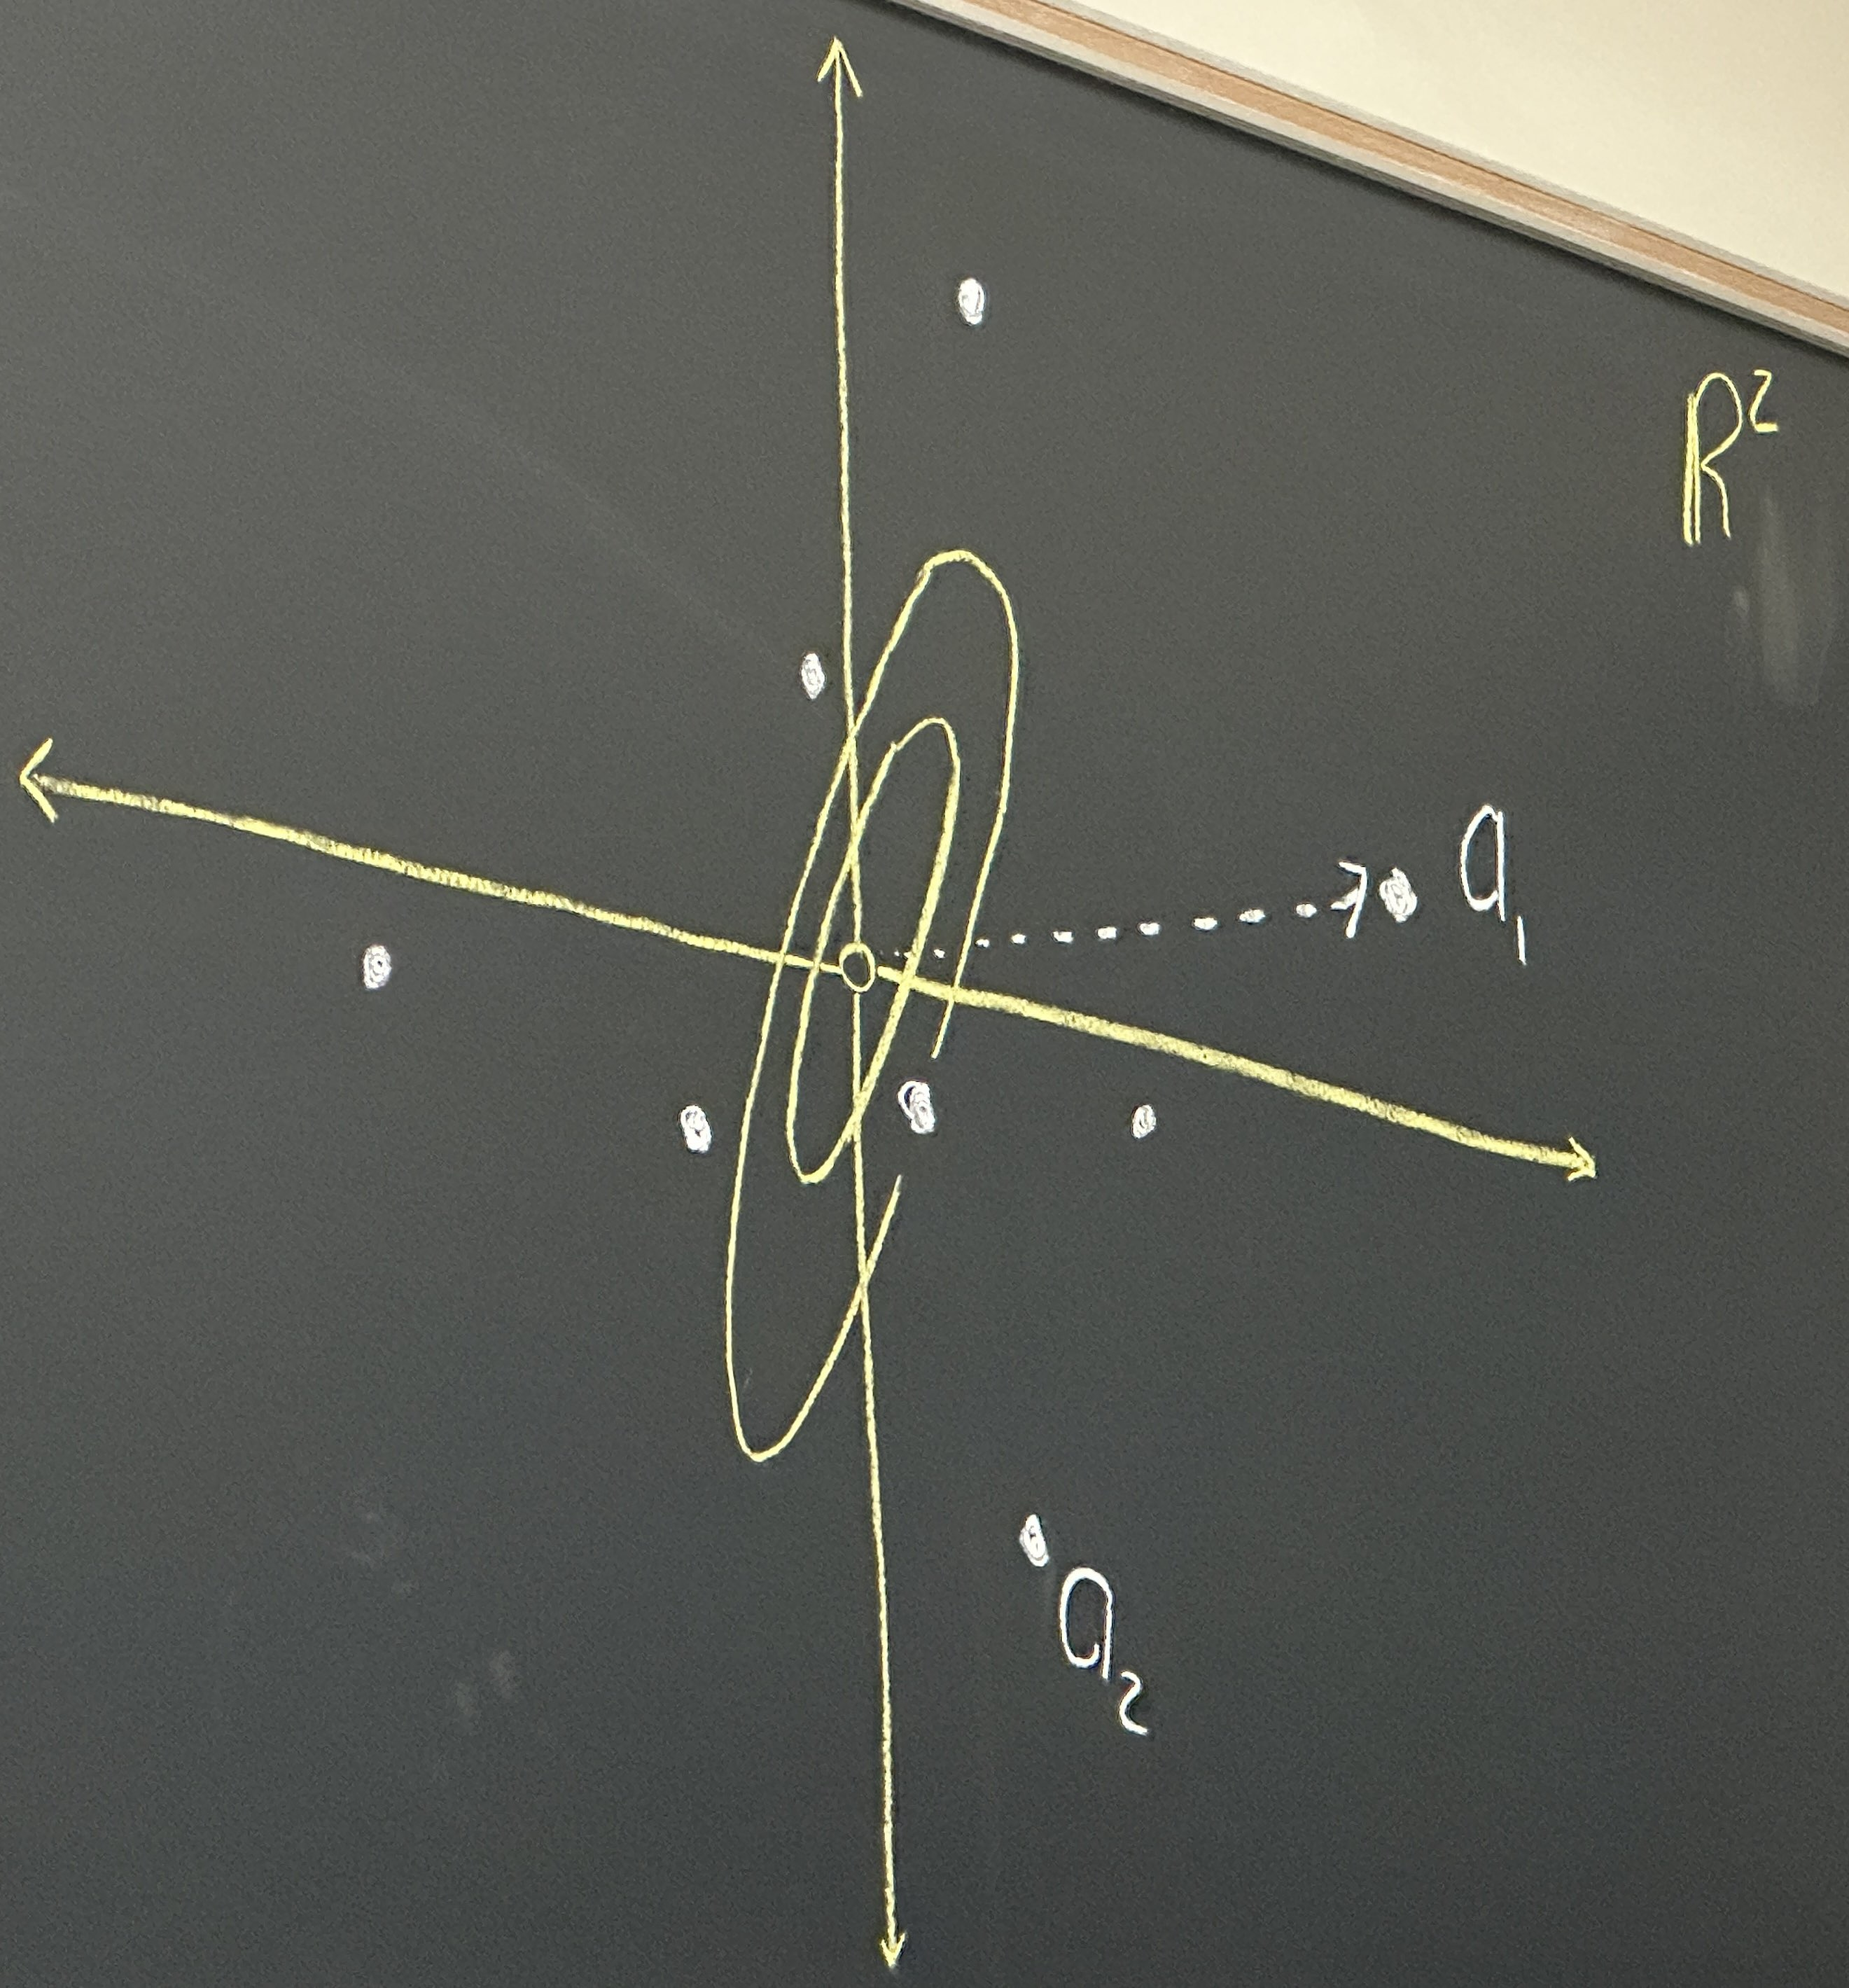
\includegraphics[scale=0.1]{lectures/wk10/img/ellipsoids.jpeg}
    \caption{Ellipsoids}
    \label{fig:ellipsoid}
\end{figure}

\subsubsection{Criteria to optimize j(n)}
\begin{enumerate}
    \item We want to choose $j$ at step $n$ to minimize $\E_{Y_n = y_n}(H[X\mid y_n, Y^{(n-1)}])=H[X\mid Y^{(n)}]$
    \item We want to choose $j(n)$ to maximize $I[X; Y^n \mid Y^{(n-1)}]$.
    \item We want to choose $j(n)$ to change your distribution the most, to maximize how much we expect the distribution to change (Information gain) after you ask the question $$\E_{Y_n = y_n}[D(\underbrace{p_{X\mid y^n, Y^{(n-1)}}}_{p_{n\mid y_n}} \| \underbrace{p_{X\mid Y^{(n-1)}}}_{p_{n-1}})]$$ where $p_{n\mid y_n}$ is the posterior and $p_{n-1}$ is the prior.
\end{enumerate}

We note that all 3 of the above criteria are equivalent. \textit{Proof:}
\begin{enumerate}
    \item Choose $j(n)\st$ it is the $\argmin_k\{\E_{Y_n(k) = y_n(k)}(H[X\mid y_n(k), Y^{(n-1)}])\}$ over all $k$th questions being asked.
    Note that this is the same as 
    $\argmin_k\{H[X\mid Y_n(k), Y^{(n-1)}]\}$
    \item $\argmin_k\{H[X\mid Y^{(n-1)}] - H[X\mid Y_n(k), Y^{(n-1)}]\}=\argmin_k\{I[X; Y_n(k)\mid Y^{(n-1)}]\}$
    Interpretation: You are greedily trying to maximize the amount of information gained.
    \item $$
    I[X; Y_n(k)\mid Y^{(n-1)}] 
    = D(p_{X, Y_n(k)\mid Y^{(n-1)}} \| \underbrace{p_{X\mid Y^{(n-1)}}}_{p_{n-1}} p_{Y_n(k)\cancel{\mid Y^{(n-1)}}})
    $$
    We started out by writing out mutual information as a KL divergence between the joint and the product of the marginals. But we note that the second marginal distribution in the product (2nd param of the KL Div.) is independent and thus can be removed. Thus we get:
    \begin{align*}
    &= \E_{X, Y_n(k)\mid Y^{(n-1)}}\left[\log\left(\frac{p_{X, Y_n(k)\mid Y^{(n-1)}}}{p_{X\mid Y^{(n-1)}} p_{Y_n(k)}}\right)\right]
    \\
    &= \E_{Y_n(k)\cancel{\mid Y^{(n-1)}}}\left[\E_{X\mid y_n, Y^{(n-1)}}\left[\log\left(\frac{p_{X, Y_n(k)\mid Y^{(n-1)}}}{p_{X\mid Y^{(n-1)}} p_{Y_n(k)}}\right)
    \right]
    \right]
    \\
    &= \E_{Y_n(k)}\left[\E_{X\mid y_n, Y^{(n-1)}}\left[\log\left(
    \frac{
        p_{Y_n(k)\mid Y^{(n-1)}}
        p_{X\mid Y_n(k), Y^{(n-1)}}
    }{p_{X\mid Y^{(n-1)}} p_{Y_n(k)}}\right)
    \right]
    \right]
    \\
    &= \E_{Y_n(k)}\left[\E_{X\mid y_n, Y^{(n-1)}}\left[\log\left(
    \frac{
        p_{Y_n(k)}
        p_{X\mid Y_n(k), Y^{(n-1)}}
    }{p_{X\mid Y^{(n-1)}} p_{Y_n(k)}}\right)
    \right]
    \right]
    \\
    &= \E_{Y_n(k)}\left[\E_{X\mid y_n, Y^{(n-1)}}\left[\log\left(
    \frac{
        p_{Y_n(k)}
        p_{X\mid Y_n(k), Y^{(n-1)}}
    }{p_{X\mid Y^{(n-1)}} p_{Y_n(k)}}\right)
    \right]
    \right]
    \\
    &= \E_{Y_n(k)}\left[\E_{X\mid y_n, Y^{(n-1)}}\left[\log\left(
    \frac{
        p_{Y_n(k)}
        p_{X\mid Y_n(k), Y^{(n-1)}}
    }{p_{X\mid Y^{(n-1)}} p_{Y_n(k)}}\right)
    \right]
    \right]
    \end{align*}
    Thus since $I[X; Y_n(k)\mid Y^{(n-1)}] = \E_{Y_n(k) = y_n(k)}[D(\underbrace{p_{n, y_n}}_{p_{X\mid y_n, Y^{(n-1)}}} \| \underbrace{p_{n-1}}_{\text{posterior given $Y^{(n-1)}$}})]$.
\end{enumerate}
Fun discussion problem: instead of an analytical solution as done below, utilize a decision tree to get an approximate solution.

Model:
$$
X\sim \cN(\mu, \Sigma_0)
$$
each question $j: q_j: a_j^\top X + \varepsilon = Y(j)$, with $\varepsilon\sim\cN(0, \sigma_j^2)$

for a fixed set of $m$ questions: $\{q_j\}_{j=1}^m$.

\begin{equation}
    q_j : Y(j) = a_j^\top X + \varepsilon
\end{equation}

This gives you a confidence interval which with high probability, you expect the true $X$ to lie when projected within the space -- you are constraining the projection of $X$ (with noise) onto a specific direction which changes the distribution. 

Since every variable in this problem is gaussian and linear, we understand how the posterior updates after each observation.

Also, a Gaussian can be uniquely identified with 2 pieces of information: $\mu, \sigma$. For a MVG, the entropy is solely dependent on the covariance matrix, so we simply need to observe how that updates.

Suppose: $p_{n-1}(X) = p(X\mid y^{(n-1)}) \sim \cN(\mu_{n-1}, \Sigma_{n-1})$.\\
Observe: $Y_{n}(j) = y_n(j) = a_j^\top X + \varepsilon$.\\
Posterior: 
\begin{align*}
p_{n}(X) 
&= p(X\mid y_n(j), y^{(n-1)}) 
\\
&\propto 
\underbrace{p_{Y_{n}{(j)}}(y_n\mid x, \cancel{Y^{(n-1)}})}_{\text{given $x$: } Y_n(j)\mid x\sim\cN(a_j^\top x, \sigma_j^2)}
p(X=x\mid y^{(n-1)})
\\
&\propto \underbrace{\exp(-\frac12 \left( 
\frac{(y-a_j^\top x)^2}{\sigma_j^2}
+
(x-\mu_{n-1})^\top \Sigma_{n-1}^{-1} (x-\mu_{n-1})
\right))}_{\ldots}
\end{align*}
where we took out the quadratic terms in $x$.

\subsubsection{Rank 1 updates to the Precision Matrix}
$$
x^\top 
\underbrace{(\frac1{\sigma_j^2}a_ja_j^\top + \Sigma_{n-1}^{-1})}_{\Sigma_0^{-1}}
x
$$

where $\Sigma_0^{-1}\implies \Sigma_n=(\Sigma_{n-1}^{-1} + \frac1{\sigma_j^2}a_ja_j^\top)^{-1}\indep Y^{(n)}$

and where $+ \frac1{\sigma_j^2}a_ja_j^\top$ is a rank 1 update to the precision, $P=\Sigma^{-1}$.

In statistics, the precision matrix or concentration matrix is the matrix inverse of the covariance matrix or dispersion matrix, $P=\Sigma^{-1}$. ${ }$ For univariate distributions, the precision matrix degenerates into a scalar precision, defined as the reciprocal of the variance, $p=\frac{1}{\sigma^2} \cdot$.

\subsubsection{Relating back to Entropy}
\vspace{-1em}
\begin{align*}
    H[X\mid Y^{(n)}] 
    &= \frac{d}2\ln(2\pi e)+\frac12\ln(\det(\Sigma_n))
    \\
    &\mapsto
    I[X; y_n(j)\mid Y^{(n-1)}]
    \\
    &= H[X\mid Y^{(n-1)}] - H[X\mid Y^{(n)}]
    \\
    &= \frac{d}2\ln(2\pi e)+\frac12\ln(\det(\Sigma_{n-1}))
    -\frac{d}2\ln(2\pi e)-\frac12\ln(\det(\Sigma_{n\mid j(n)}))
    \\
    &= \frac12\ln(\frac{\det(\Sigma_{n-1})}{\det(\Sigma_{n\mid j(n)})})
\end{align*}

Note that:
\begin{align*}
& \det\left(\Sigma_{n-1}^{1 / 2} \Sigma_{n \mid j(n)}^{-1} \Sigma_{n-1}^{1 / 2}\right) \\
& \det\left(\Sigma_{n-1}^{1 / 2}\left(\Sigma_{n-1}^{-1}+\frac{1}{\sigma_j^2} a_ja_j^\top\right) \Sigma_n^{1 / 2}\right) \\
& \det\left(I+\frac{1}{\sigma_j}\left({\Sigma}_n^{1 / 2} a_j\right)\left({\Sigma}_n^{\frac{1}{2}} a_j^{\top}\right)\right)
\end{align*}

\begin{figure}[H]
    \centering
    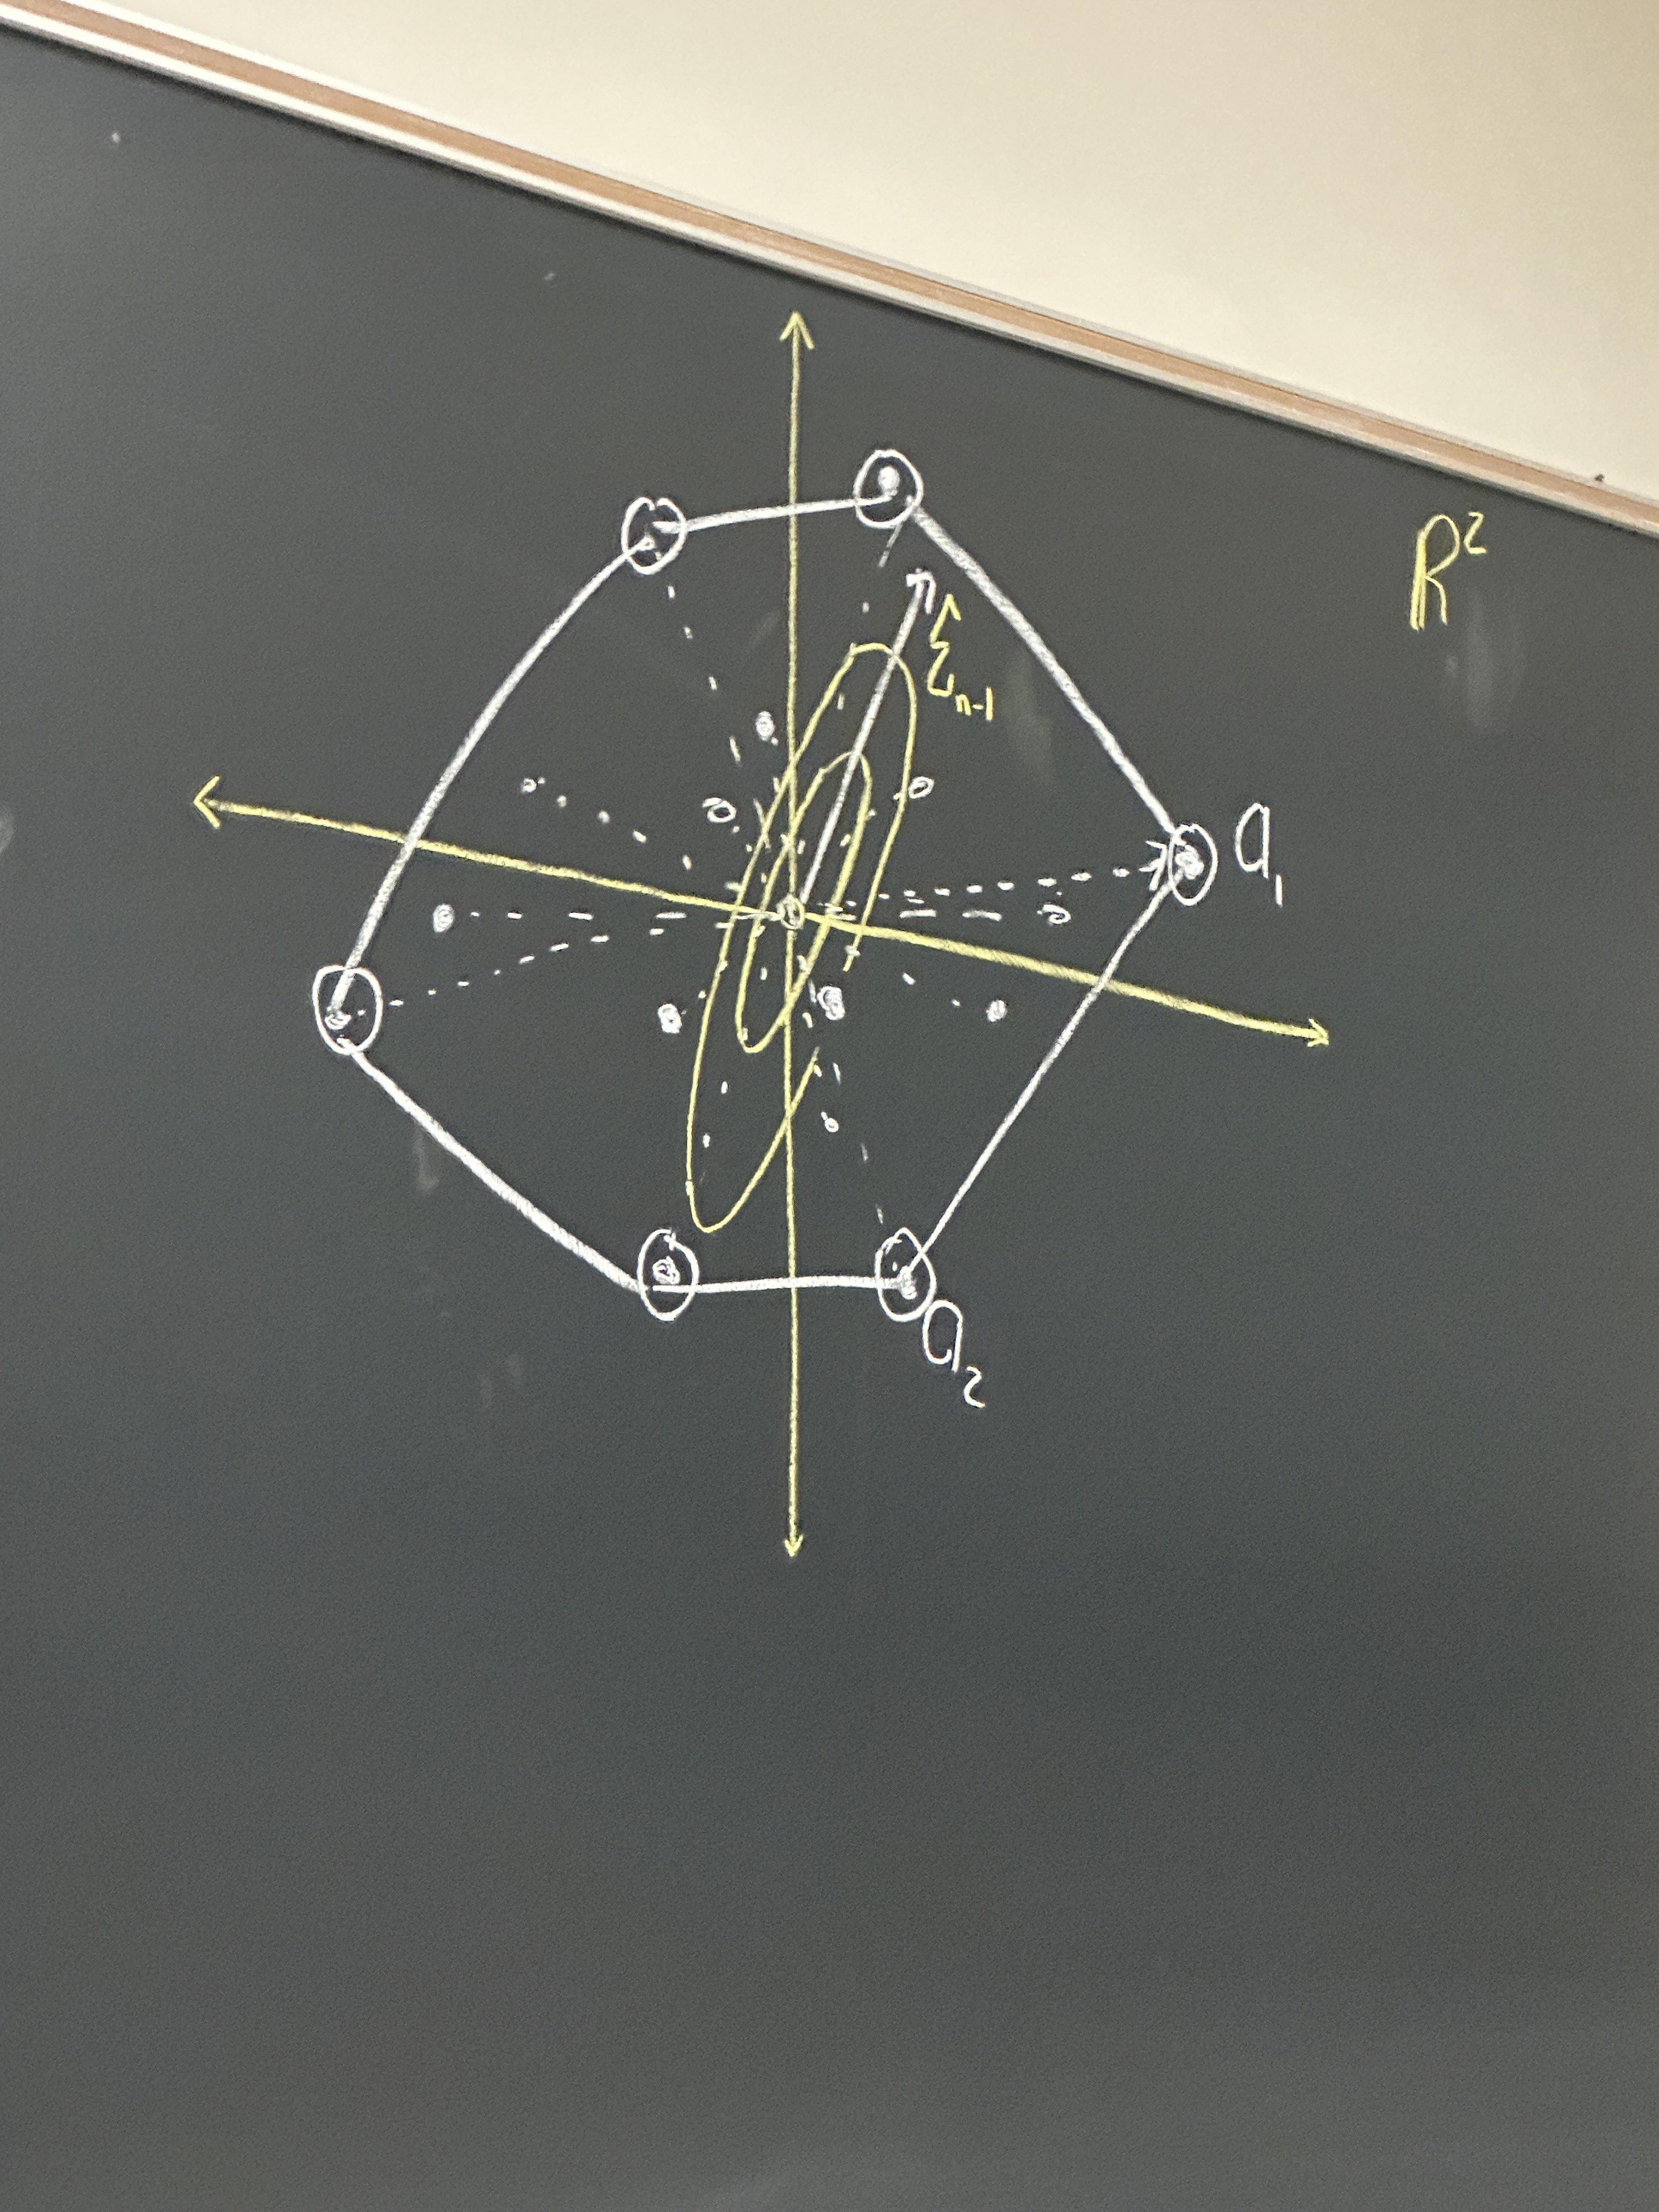
\includegraphics[scale=0.1]{lectures/wk10/img/constrainedEllipsoid.jpeg}
    \caption{Constrained Ellipsoid}
    \label{fig:constrained-ellipsoid}
\end{figure}

\subsection{Quadratic Programming is a Geometry Problem}
\begin{figure}[H]
    \centering
    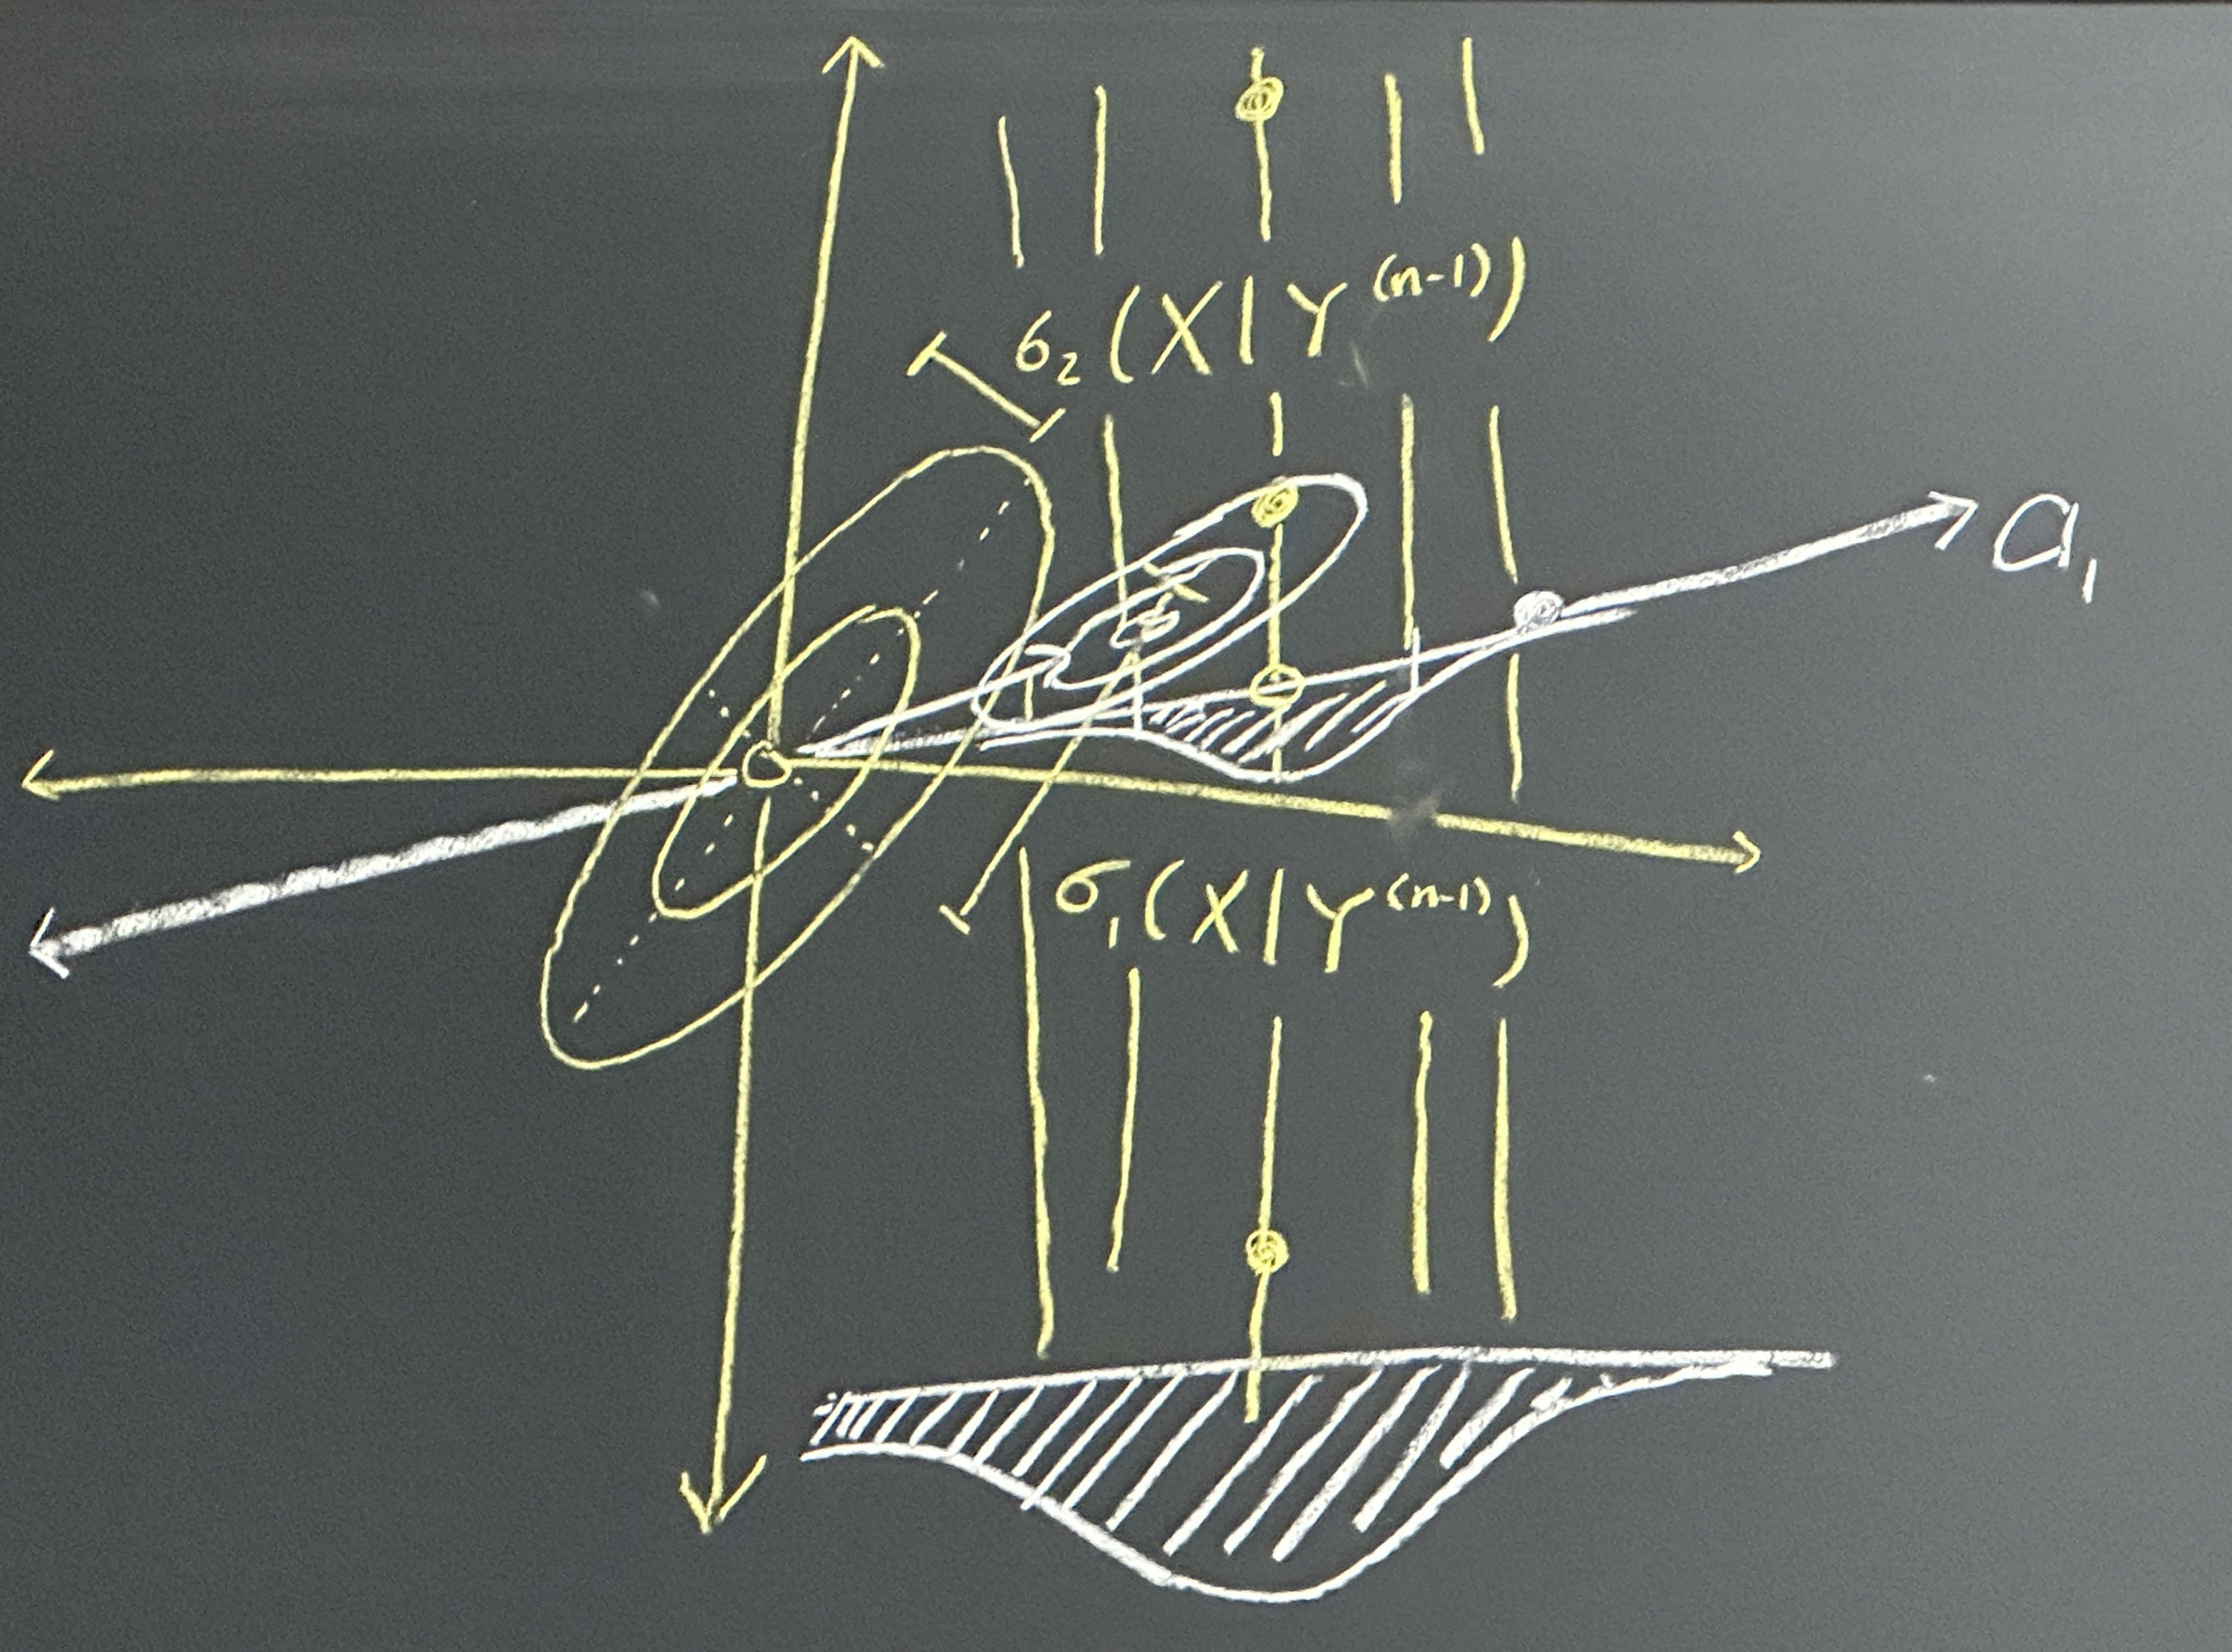
\includegraphics[scale=0.1]{lectures/wk10/img/QP.jpeg}
    \caption{Quadratic Program}
    \label{fig:quadratic-rogram}
\end{figure}
$$
\lambda_i(I+A)=1+\lambda_i(A)
$$

$$
\left(u u^{\top}\right)=
\begin{bmatrix}
    \\
    u
    \\ 
    \\
\end{bmatrix}
\begin{bmatrix}
  \quad  & u^\top & \quad
\end{bmatrix}
$$

\begin{itemize}
    \item Acquisition: pick $j(n)=\argmax_k \{\frac1\sigma_k^2 a_k^\top \Sigma_{n-1} a_k\}$
    \item Quadratic programming on a discrete set
\end{itemize}

\begin{equation}
\left(u u^{\top}\right) u=u\left(u^{\top} u\right)=\underbrace{\|u\|^2 u}_\lambda
\end{equation}
